\documentclass[12pt,a4paper]{article}
\usepackage[utf8]{inputenc}
\usepackage{dsfont} 
\usepackage[polish]{babel}
\usepackage{amsmath}
\usepackage{graphicx}
\usepackage[top=1in, bottom=1.5in, left=1.25in, right=1.25in]{geometry}

\usepackage{subfig}
\usepackage{multirow}
\usepackage{multicol}
\graphicspath{{Imagens/}}
\usepackage{xcolor,colortbl}
\usepackage{float}

\newcommand \comment[1]{\textbf{\textcolor{red}{#1}}}

%\usepackage{float}
\usepackage{fancyhdr} % Required for custom headers
\usepackage{lastpage} % Required to determine the last page for the footer
\usepackage{extramarks} % Required for headers and footers
\usepackage{indentfirst}
\usepackage{placeins}
\usepackage{scalefnt}
\usepackage{xcolor,listings}
\usepackage{textcomp}
\usepackage{color}
\usepackage{verbatim}
\usepackage{framed}

\definecolor{codegreen}{rgb}{0,0.6,0}
\definecolor{codegray}{rgb}{0.5,0.5,0.5}
\definecolor{codepurple}{HTML}{C42043}
\definecolor{backcolour}{HTML}{F2F2F2}
\definecolor{bookColor}{cmyk}{0,0,0,0.90}  
\color{bookColor}

\lstset{upquote=true}

\lstdefinestyle{mystyle}{
	backgroundcolor=\color{backcolour},   
	commentstyle=\color{codegreen},
	keywordstyle=\color{codepurple},
	numberstyle=\numberstyle,
	stringstyle=\color{codepurple},
	basicstyle=\footnotesize\ttfamily,
	breakatwhitespace=false,
	breaklines=true,
	captionpos=b,
	keepspaces=true,
	numbers=left,
	numbersep=10pt,
	showspaces=false,
	showstringspaces=false,
	showtabs=false,
}
\lstset{style=mystyle}

\newcommand\numberstyle[1]{%
	\footnotesize
	\color{codegray}%
	\ttfamily
	\ifnum#1<10 0\fi#1 |%
}

\definecolor{shadecolor}{HTML}{F2F2F2}

\newenvironment{sqltable}%
{\snugshade\verbatim}%
{\endverbatim\endsnugshade}

% Margins
\addtolength{\footskip}{0cm}
\addtolength{\textwidth}{1.4cm}
\addtolength{\oddsidemargin}{-.7cm}

\addtolength{\textheight}{1.6cm}
%\addtolength{\topmargin}{-2cm}

% paragrafo
\addtolength{\parskip}{.2cm}

% Set up the header and footer
\pagestyle{fancy}
\rhead{\hmwkAuthorName} % Top left header
\lhead{\hmwkClass: \hmwkTitle} % Top center header
\rhead{\firstxmark} % Top right header
\lfoot{Piotr Włodarczak} % Bottom left footer
\cfoot{} % Bottom center footer
\rfoot{} % Bottom right footer
\renewcommand{\headrulewidth}{1pt}
\renewcommand{\footrulewidth}{1pt}

    
\newcommand{\hmwkTitle}{Hotelowa baza danych MySQL} % Tytuł projektu
\newcommand{\hmwkDueDate}{24.05.2020} % Data 
\newcommand{\hmwkClass}{Bazy danych} % Nazwa przedmiotu
\newcommand{\hmwkAuthorName}{Piotr Włodarczak} % Imię i nazwisko

% trabalho 
\begin{document}
% capa
\begin{titlepage}
    \vfill
	\begin{center}
	\hspace*{-1cm}
	\vspace*{0.5cm}
	\textbf{Uniwersytet Gdański \\ [0.05cm]Wydział Matematyki, Fizyki i Informatyki \\ [0.05cm] Instytut Informatyki}

	\vspace{0.6cm}
	\vspace{4cm}
	{\huge \textbf{\hmwkTitle}}\vspace{8mm}
	
	{\large \textbf{\hmwkAuthorName}}\\[3cm]
	
		\hspace{.45\textwidth} %posiciona a minipage
	   \begin{minipage}{.5\textwidth}
	   Projekt z przedmiotu bazy danych na kierunku informatyka profil ogólnoakademicki na Uniwersytecie Gdańskim.\\[0.1cm]
	  \end{minipage}
	  \vfill
	%\vspace{2cm}
	
	\textbf{Gdańsk}
	
	\textbf{\hmwkDueDate}
	\end{center}
	
\end{titlepage}

\newpage
\setcounter{secnumdepth}{5}
\tableofcontents
\newpage

\section{Wprowadzenie}
\label{sec:introduction}

Powstała baza danych ma na celu ułatwienie zarządzania hotelami, pensjonatami i ośrodkami wypoczynkowymi, poprzez łatwą i przejrzystą rejestrację rezerwacji, organizację dostępnych miejsc i przekazywania informacji o ośrodku klientom. 

\section{Opis projektu}
\label{sec:Project}

Projekt powstał jako uniwersalne rozwiązanie dla firm przechodzących informatyzację baz danych, z papierowych katalogów i kalendarzy w innowacyjne komputerowe systemy bazodanowe, minimalizujące możliwość popełniania błędów w rezerwacjach i usprawniające działanie personelu recepcyjnego. Ułatwia on także korzystanie z bazy hoteli klientom, którzy mogą za jej pomocą sprawdzić różne parametry hotelu, takie jak jego lokalizacja, miejsca parkingowe czy możliwość wprowadzenia się ze zwierzętami


\subsection{Potencjalne grupy użytkowników}
\label{sec:Users}

\begin{itemize}
	\item Administrator – główny zarządca bazy danych, posiada pełen dostęp do bazy danych, może modyfikować dowolne elementy systemu.
	\item Recepcjonista - może tworzyć rezerwacje, sprawdzać historię rezerwacji pokojów, potwierdzać rezerwacje i porównywać dane klienta z danymi podanymi przy rezerwacji w celu potwierdzenia tożsamości
	\item Klient - może dostosować hotel do swoich potrzeb, sprawdzając czy na terenie obiektu znajdują się potrzebne mu udogodnienia, czy są wolne pokoje lub jakie hotele występują w danej lokalizacji, nie może wprowadzać zmian w bazach danych
	\item Zarząd - zarząd ośrodka jest w stanie, na podstawie analizy najczęściej rezerwowanych pokojów, najpopularniejszych ofert i demografii klientów, wyciągać wnioski pozwalające na tworzenie ofert lepiej dostosowanych do klientów lub modyfikacje ośrodka w oparciu o trendy rynkowe
	\item Służby ratownicze - w wypadku pożaru, trzęsienia ziemii lub innego nieprzewidzianego wypadku oszacowanie ilości i zidentyfikowanie znajdujących się w hotelu osób powinno być bezpieczne i szybkie
	
\end{itemize}
\newpage
\subsection{Wymagania funkcjonalne}
\label{sec:FunctionalConditions}

Dane które będzie przechowywała baza danych:
\begin{itemize}
    \item Personalne dane klientów
    \item Oferty hoteli
    \item Lista hoteli w danej lokalizacji
\end{itemize}

Do jakich zadań baza danych będzie używana

\begin{itemize}
    \item Rezerwacje poszczególnych pokoi
    \item Potwierdzanie danych klienta z danymi podanymi przy rezerwacji
    \item Sprawdzanie ofert hoteli
\end{itemize}

\subsection{Wymagania niefunkcjonalne}
\label{sec:NonFunctionalConditions}

Baza danych stworzona jest w MySQL, który jest jednym z najszybszych dostępnych narzędzi tworzenia baz dancyh. W porównaniu do innych wersji jest wybitnie wydajny, sprawny, a także prosty i przejrzysty. MySQL jest także bardzo bezpiecznym narzędziem - administrator bazy danych może zarządzać uprawnieniami, decydować o tym jakie zmiany mogą być przeprowadzane w bazie danych a jakie nie.
\newline
\newline
Jednakże, wadami tego rozwiązania jest zwiększone zużycie pamięci, a także trudności w ewentualnym debugowaniu i utrzymywaniu bazy danych w dobrym stanie.

\subsection{Diagram związków encji}
\label{sec:ERD} 

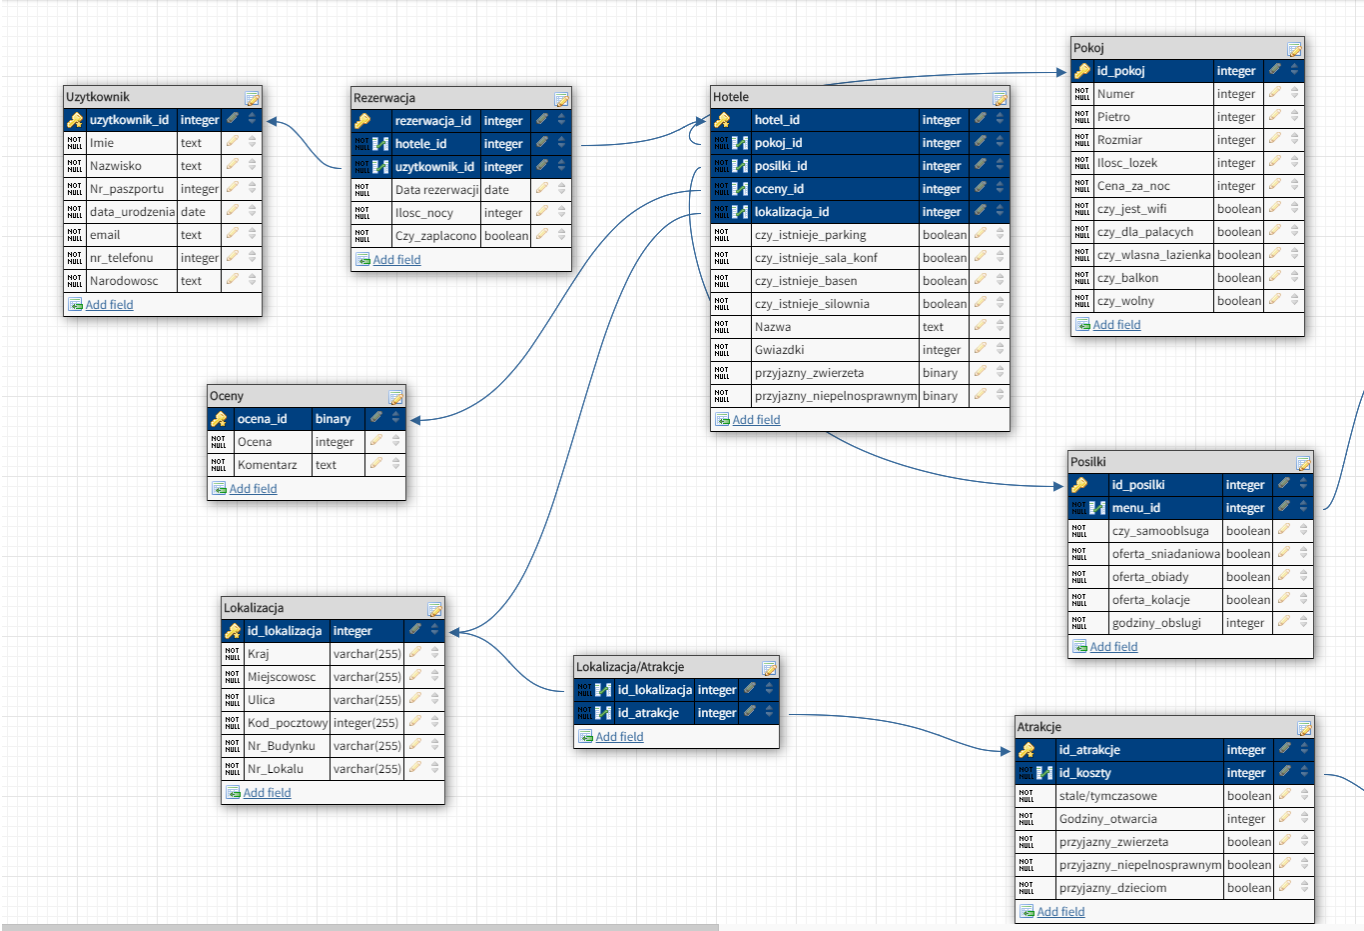
\includegraphics[angle=0,width=160mm,height=100mm]{img/erd3.png}
\newline
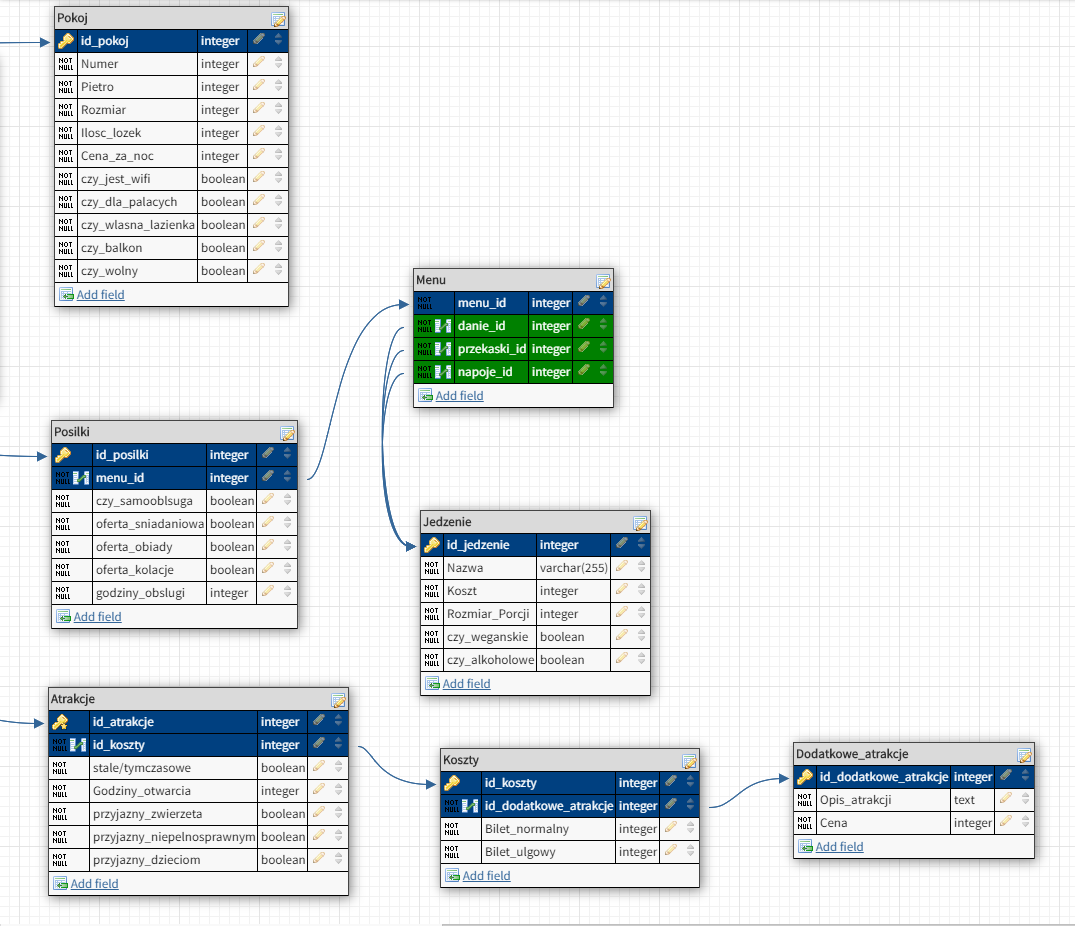
\includegraphics[angle=0,width=150mm,height=120mm]{img/erd4.png}

\section{Przykłady realizacji bazy danych}
\label{sec:ExamplesSection}
Niżej zaprezentowane przykłady dotyczą tabeli Pokój, przechowującej dane dla poszczególnych pokojów, oraz pytania o pokoje znajdujące się w danym hotelu
\subsection{Przykłady zawartości najważniejszych tabel}
Tabela Pokoj, odpowiedzialna za przechowywanie danych konkretnego pokoju
\newline
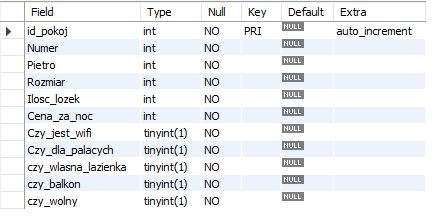
\includegraphics[angle=0,width=160mm,height=90mm]{img/tabela1.png}
\newline
Tabela Hotel, odpowiedzialna za przechowywanie danych konkretnego hotelu
\newline
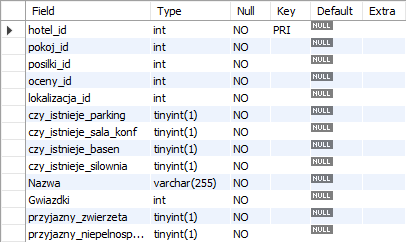
\includegraphics[angle=0,width=160mm,height=90mm]{img/tabela2.png}
\subsection{Przykłady kilku zapytań i ich wyników}

Najtansze pokoje posiadajace wifi w danym hotelu

\begin{lstlisting}[language=SQL]
SELECT * FROM pokoj WHERE Czy_jest_wifi = TRUE
ORDER BY Cena_za_noc
\end{lstlisting}
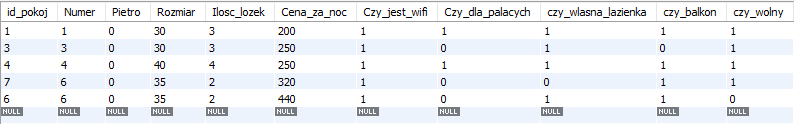
\includegraphics[angle=0,width=150mm,height=25mm]{img/result2.png}
Wolne pokoje dla palących

\begin{lstlisting}[language=SQL]
SELECT * FROM pokoj WHERE Czy_dla_palacych = TRUE AND Czy_wolny = TRUE
\end{lstlisting}
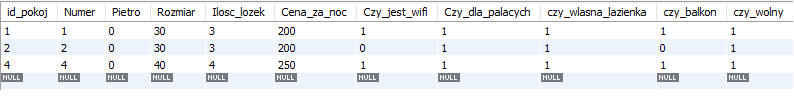
\includegraphics[angle=0,width=150mm,height=25mm]{img/result1.png}

\noindent
\bibliographystyle{amsplain}
\bibliography{references.bib}
\nocite{*}

\end{document}